%-----------------Default settings-------------------%
\documentclass[dvipsnames, aspectratio = 169]{beamer}
\usetheme{Madrid}
\usepackage{color}
\usecolortheme{default}

%----------Graphics and multimedia packages----------%
\usepackage{graphicx}
\graphicspath{{images/}}
\usepackage{multimedia}

%----------Math and Physics packages----------%
\usepackage{amssymb}
\usepackage{amsmath}
\usepackage{physics}
\usepackage{mathtools}

%---------------Useful Packages---------------%
\usepackage{tabulary}
\usepackage{hyperref}
\setbeamertemplate{caption}[numbered]
\newcommand*\df{\mathop{}\!\mathrm{d}}
\newcommand*\Df[1]{\mathop{}\!\mathrm{d^#1}}

%-------------Set Bibliography---------------%
\usepackage{natbib}
\bibliographystyle{ksfh_nat}

\title[Master's Thesis]{A conceptual study of the combined effect of flutter and friction}
\author[Javier Luis González Monge]{\textbf{Author:} Javier Luis González Monge\\
{\small \textbf{Advisor:} }}
\institute[]{\large Máster Universitario en Sistemas Espaciales \\
	{\large Technical University of Madrid}}
\titlegraphic{%
	\makebox[0.8\paperwidth]{%
		
\includegraphics[width=2.5cm,keepaspectratio]{Upmlogo.pdf}%
		\hfill
		
\includegraphics[width=2.0cm,keepaspectratio]{idr.png}%
		\hfill
		
\includegraphics[width=2.5cm,keepaspectratio]{etsiae.png}%
	}%
}

\begin{document}


\begin{frame}
	\maketitle
\end{frame}


\begin{frame}
	\frametitle{Outline}
	\tableofcontents
\end{frame}

\section{Introduction}

%  	\begin{frame}{Introduction}
%  		\begin{columns}
%  			\begin{column}{0.5\textwidth}
%  				\begin{itemize}
%  					\item The vibration of the blades of a LPT (Low Pressure Turbine) rotor is an \textbf{aeroelastic} problem
%  					\item This problem is enclosed in the center of Collar's Triangle 
% 					\item Flutter and friction at the fir tree union are two fundamental effects that define the final state of the system
%  				\end{itemize}
%  			\end{column}
%  			\begin{column}{0.5\textwidth}
%  				\begin{figure}[h!]
%  					\centering
%  					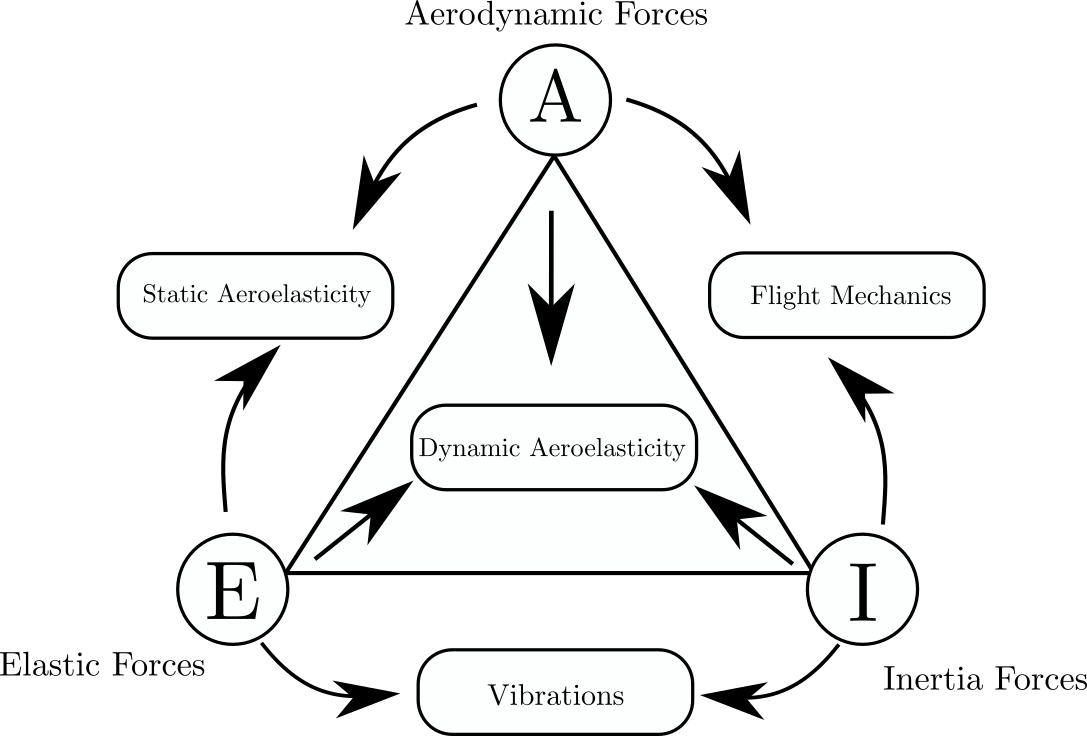
\includegraphics[width = 1\textwidth]{Collar.png}
%  					\caption{Collar's Triangle (\cite{collar1946expanding})}
%  					\label{collaar}
%  				\end{figure}
%  			\end{column}		
%  		\end{columns}
%  	\end{frame}

\begin{frame}{Introduction}
	\begin{columns}
		\begin{column}{0.5\textwidth}
			\begin{itemize}
				\item Flutter is an aeroelastic instability
				\item Flutter onset is a linear effect (due to small displacements)
				\item The amplitude of the blades grow exponentially because of this instability
				\item Non-linear friction at the fir-tree saturates the instability. The amplitude of vibration is bounded
				\item There are two time scales in this problem
				      \begin{enumerate}
					      \item Fast elastic oscillations of the blade
					      \item Amplitude modulation by the effect of flutter and friction
				      \end{enumerate}
			\end{itemize}
		\end{column}
		\begin{column}{0.5\textwidth}
			\begin{figure}[h!]
				\centering
				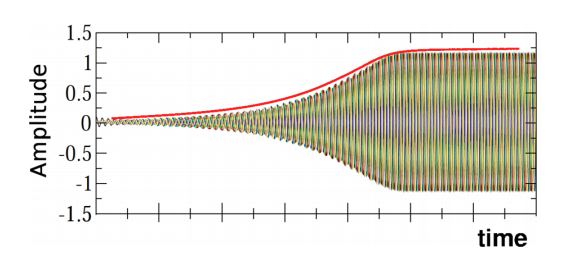
\includegraphics[width = 0.9\textwidth]{amplitude.png}
				\caption{Evolution of the blade vibration amplitude over time (Martel, Corral, Rahul (2015))}
				\label{fig:amplitude_fast_oscillation}
			\end{figure}
		\end{column}
	\end{columns}
\end{frame}

\section{Bladed-disk Problem}
\begin{frame}{Bladed-disk Problem}
	\begin{columns}
		\begin{column}{0.5\textwidth}
			\begin{itemize}
				\item A realistic FEM model has around 5,000,000 DOF
				\item The system of equations of the bladed-disk is
			\end{itemize}

			\begin{equation}\label{eq:general_bladed-disk}
				[M]\{\ddot{X}\} + [C]\{\dot{X}\} + [K]\{X\} + \{F_{nl}\} + \{F_a\} = 0,
			\end{equation}
			\begin{itemize}
				\item This model is computationally expensive
				\item An asymptotic ROM is convenient to study the qualitative behaviour
			\end{itemize}
		\end{column}
		\begin{column}{0.5\textwidth}
			\begin{figure}[h!]
				\centering
				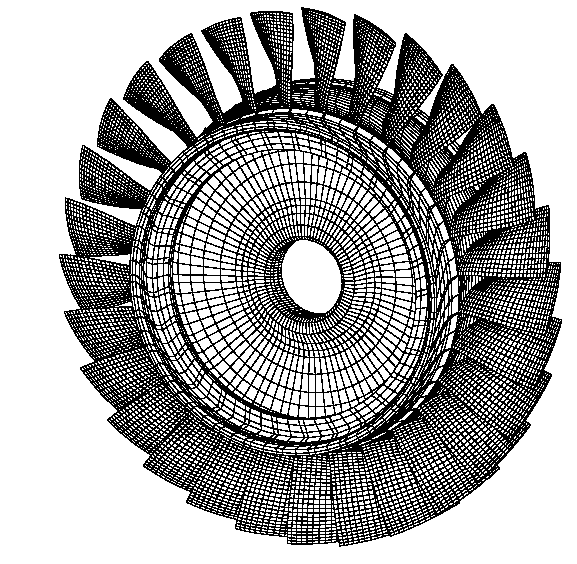
\includegraphics[width = 0.6\textwidth]{Bladed_disk.png}
				\caption{Bladed-disk FEM model}
				\label{fig:rotationsymmetry}
			\end{figure}
		\end{column}
	\end{columns}
\end{frame}



\section{Asymptotic Reduced Order Model}

\begin{frame}{Asymptotic Reduced Order Model}
	\begin{figure}[h!]
		\centering
		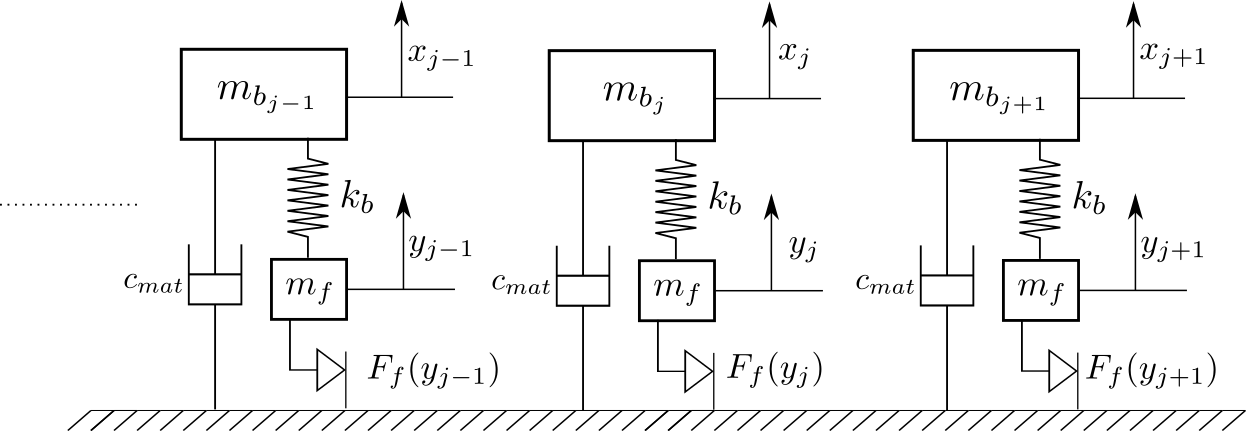
\includegraphics[width = 0.75\textwidth]{mass_spring_model.png}
		\caption{Mass-spring model}
	\end{figure}
	\begin{equation}\label{eq:gen_xj}
		(m_b [I] + [·m]_D)\{\ddot{x}\} + k_b(\{x\}-\{y\}) + [\mathrm{K_c}]\{x\} + c_{mat}\{\dot{x}\} + \{F_{aero}\} = \{F_l\},
	\end{equation}
	\begin{equation}\label{eq:gen_yj}
		m_f\{\ddot{y}\} + k_b(\{y\} - \{x\}) + \{F_f(\{y\})\} = \{0\}.
	\end{equation}
\end{frame}

\begin{frame}{Asymptotic Reduced Order Model}
	\begin{itemize}
		\item A multiple scales asymptotic technique is used to filter the fast elastic oscillations
		\item Only solve for the envelope of the displacements
		\item Remove numerical stiffness from the problem
		\item The structure and aero matrices are circulant. Therefore the system is diagonalizable by performing the DFT (except the friction matrix)
		\item The change to between displacements and TW (Traveling Wave) amplitudes is $ X = [E]A $. The dimensionless equations for the asymptotic ROM are
	\end{itemize}
	\begin{equation}\label{eq:tuned_TW_Basis_system}
		\begin{split}
			2i\frac{\df}{\df \tau}&\begin{pmatrix}
				\vdots \\
				A_j    \\
				\vdots
			\end{pmatrix}
			= [E]^H\begin{bmatrix}
				Q(|X_1|) & \cdots & 0        \\
				\vdots   & \ddots & \vdots   \\
				0        & \cdots & Q(|X_N|)
			\end{bmatrix}[E]\begin{pmatrix}
				\vdots \\
				A_j    \\
				\vdots
			\end{pmatrix}\\
			&- 2\left(\begin{bmatrix}
					\frac{·\omega_1 + \eta_a^1}{\theta} & \cdots & 0                                   \\
					\vdots                              & \ddots & \vdots                              \\
					0                                   & \cdots & \frac{·\omega_N + \eta_a^N}{\theta}
				\end{bmatrix}
			+ i \begin{bmatrix}
					\frac{\xi_{mat} + \xi_a^1}{\theta} & \cdots & 0                                  \\
					\vdots                             & \ddots & \vdots                             \\
					0                                  & \cdots & \frac{\xi_{mat} + \xi_a^N}{\theta}
				\end{bmatrix}
			\right)\begin{pmatrix}
				\vdots \\
				A_j    \\
				\vdots
			\end{pmatrix}.
		\end{split}
	\end{equation}
\end{frame}

\begin{frame}{Asymptotic Reduced Order Model}
	\begin{itemize}
		\item For a system with 24 blades
	\end{itemize}
	\begin{columns}
		\begin{column}{0.5\textwidth}
			\begin{figure}[h!]
				\centering
				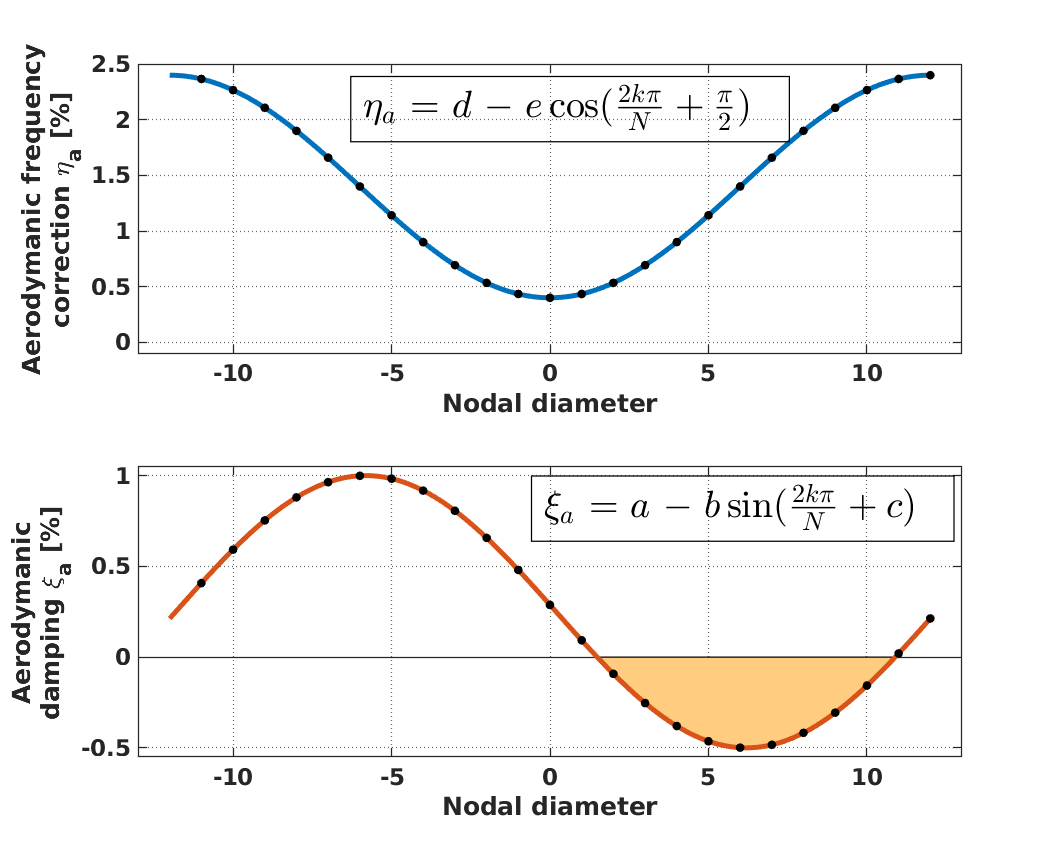
\includegraphics[width = 0.9\textwidth]{aerodynamic_coefficients.png}
				\caption{Aerodynamic coefficients}
				\label{fig:aerocoeff}
			\end{figure}
		\end{column}
		\begin{column}{0.5\textwidth}
			\begin{figure}[h!]
				\centering
				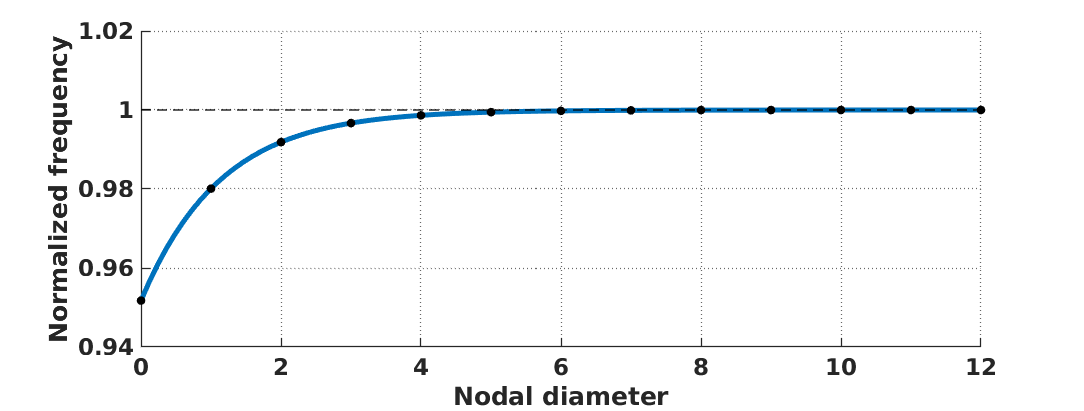
\includegraphics[width = 0.9\textwidth]{omega_distribution.png}
				\label{fig:omega_distribution}
				\caption{Frequency distribution of the first modal family}
			\end{figure}
		\end{column}
	\end{columns}
\end{frame}
\begin{frame}{Asymptotic Reduced Order Model}
	\begin{columns}
		\begin{column}{0.5\textwidth}
			\begin{figure}[h!]
				\centering
				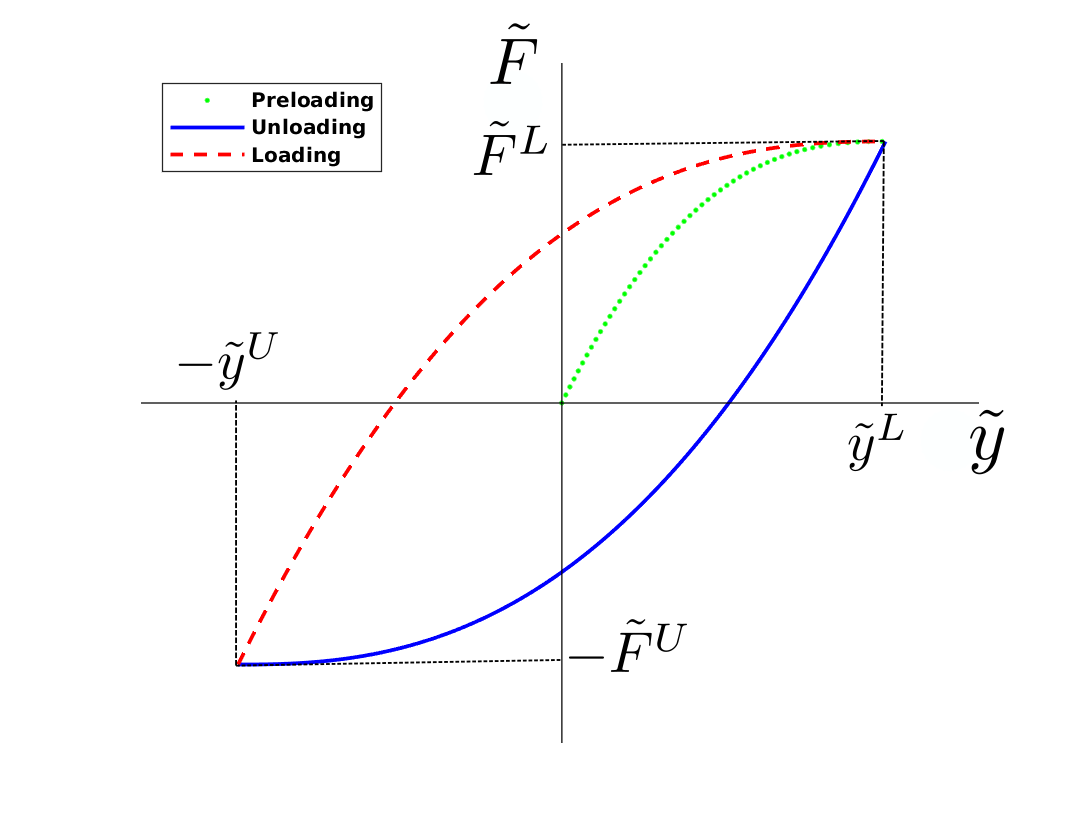
\includegraphics[width = 0.9\textwidth]{hysteresis_loop.png}
				\label{fig:omega_distributiona}
				\caption{Friction force hysteresis loop. Microslip regime (Olofsson (1996))}
			\end{figure}
		\end{column}
		\begin{column}{0.5\textwidth}
			\begin{figure}[h!]
				\centering
				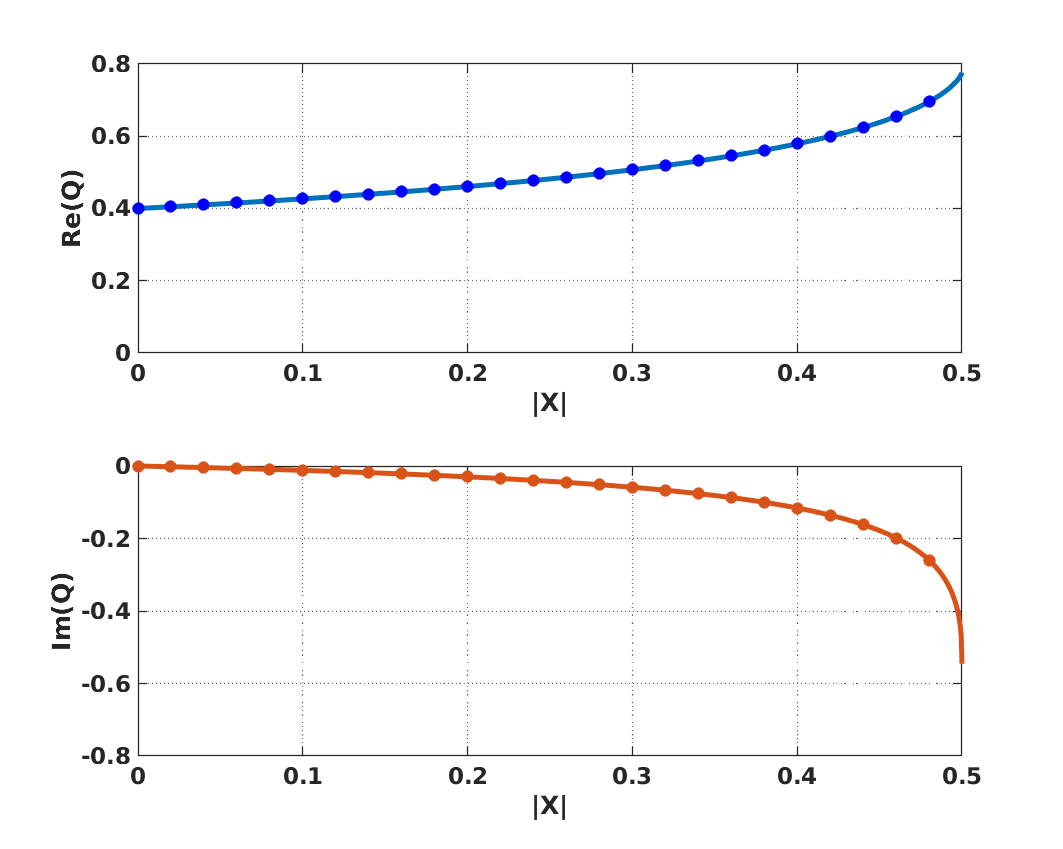
\includegraphics[width = 0.9\textwidth]{friction_oloffson_coeff.png}
				\caption{Complex friction coefficient}
				\label{fig:complefric}
			\end{figure}
		\end{column}
	\end{columns}
\end{frame}

\begin{frame}{Asymptotic Reduced Order Model}
	\begin{itemize}
		\item The solution of the system with initial condition $ A_j = 0.1 $ for $ j = 1,...,N $ is
	\end{itemize}
	\begin{columns}
		\begin{column}{0.5\textwidth}
			\begin{figure}[h]
				\centering
				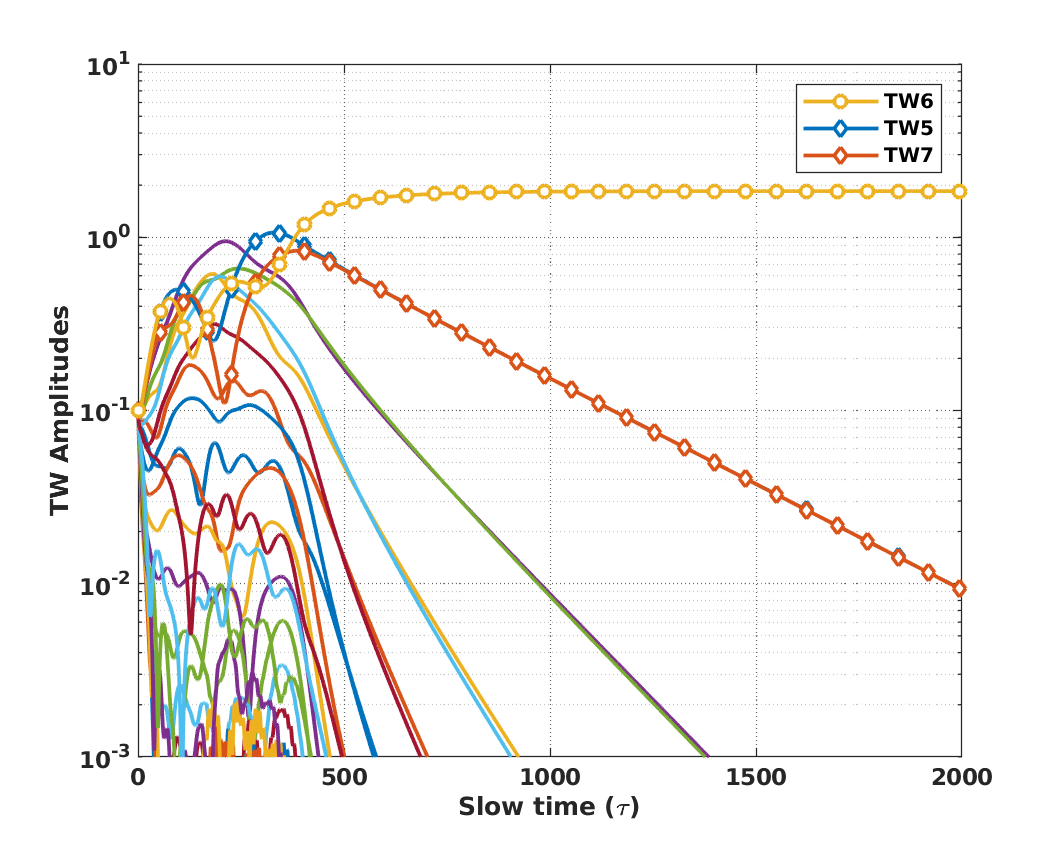
\includegraphics[width = 0.9\textwidth]{log_TW_amplitude.png}
				\caption{TW amplitude evolution (log scale)}
				\label{fig:log_TW_amp_base}
			\end{figure}
		\end{column}
		\begin{column}{0.5\textwidth}
			\begin{figure}[h]
				\centering
				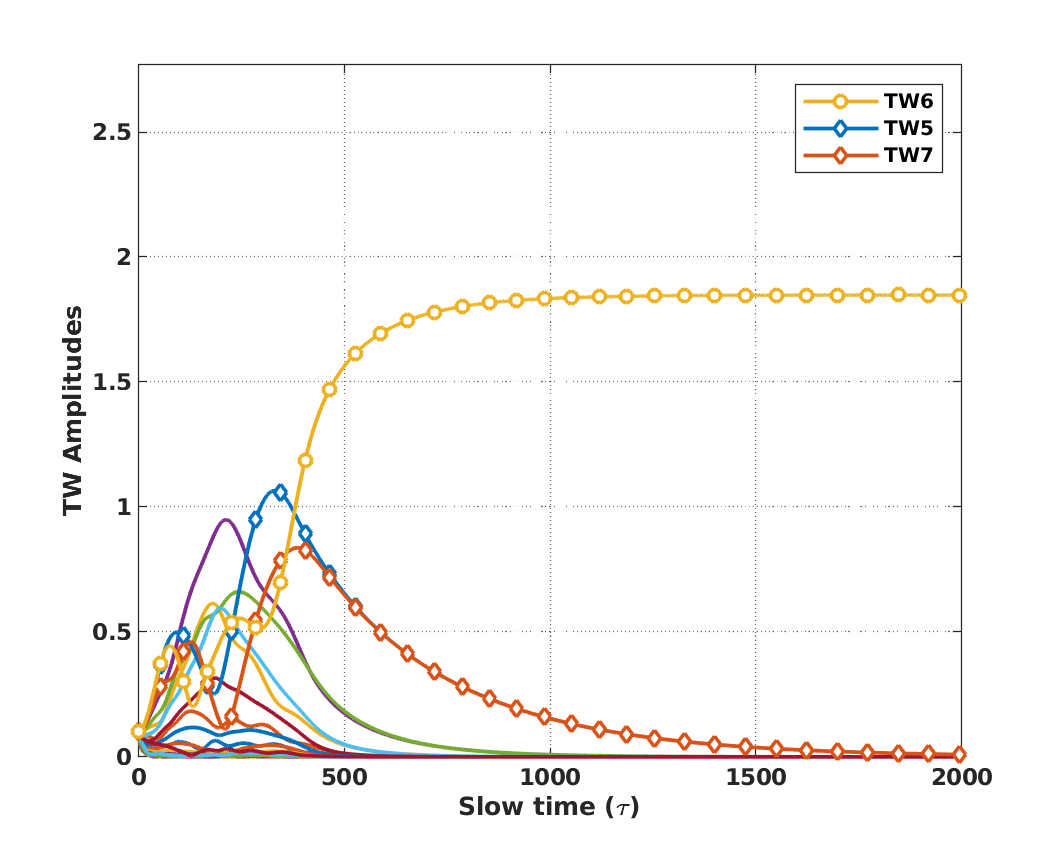
\includegraphics[width = 0.9\textwidth]{TW_amplitude.png}
				\caption{TW amplitude evolution (linear scale)}
				\label{fig:TW_amp_base1}
			\end{figure}
		\end{column}
	\end{columns}
\end{frame}

\begin{frame}{Asymptotic Reduced Order Model}
	\begin{columns}
		\begin{column}{0.48\textwidth}
			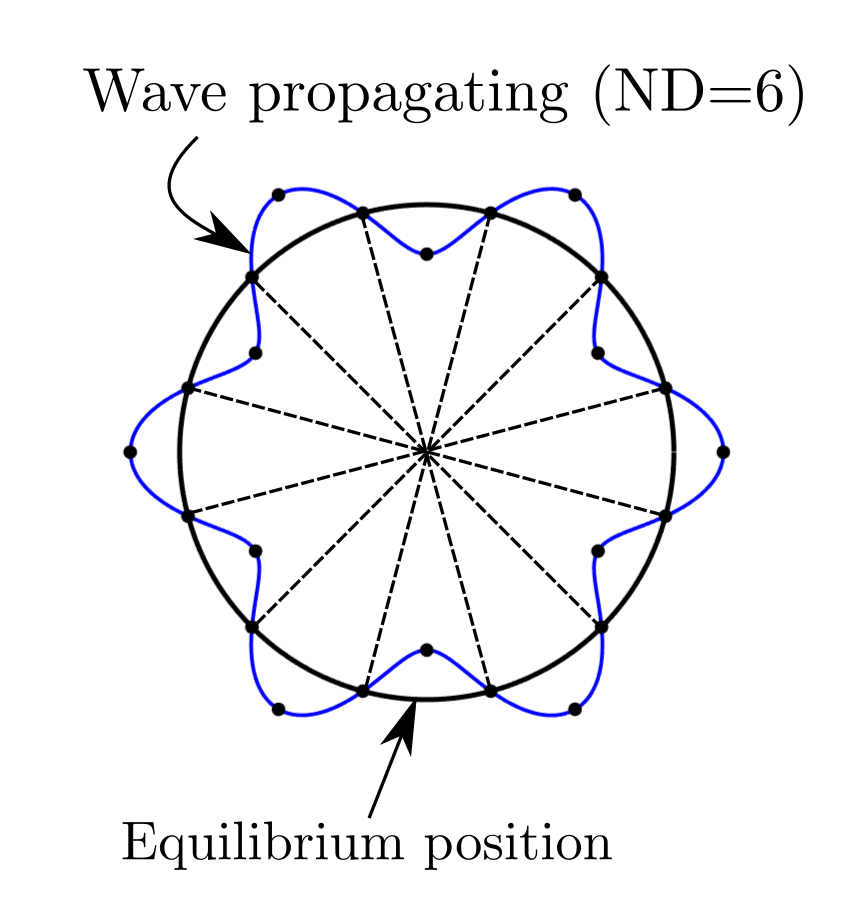
\includegraphics[width=6.5cm,keepaspectratio]{Mode_shapeND6.png}
		\end{column}
		%			\begin{column}{0.48\textwidth}
		%				\movie[width=7cm, height=4.8cm]{\includegraphics[width=7cm, height=4.7cm]{SingleWave.jpeg}}{Images/PureTW.avi}
		%			\end{column}		
	\end{columns}
\end{frame}


\section{Stability Analysis}

\begin{frame}{Stability Analysis}{Trivial Solution}
	\begin{itemize}
		\item The linear system around the trivial solution $ A = 0 $ is
	\end{itemize}

	\begin{equation}\label{eq:trivial_solution_equilibria}
		\frac{\df}{\df \tau}\begin{pmatrix}
			\vdots \\
			a_j    \\
			\vdots
		\end{pmatrix}
		=  \begin{bmatrix}
			-\frac{\xi_{mat} + \xi_a^1}{\theta} + i\left(\frac{·\omega_1 + \eta_a^1}{\theta}-\frac{\real{[Q(0)]}}{2}\right) & \cdots & 0                                                                                                               \\
			\vdots                                                                                                          & \ddots & \vdots                                                                                                          \\
			0                                                                                                               & \cdots & -\frac{\xi_{mat} + \xi_a^N}{\theta} + i\left(\frac{·\omega_N + \eta_a^N}{\theta}-\frac{\real{[Q(0)]}}{2}\right)
		\end{bmatrix}
		\begin{pmatrix}
			\vdots \\
			a_j    \\
			\vdots
		\end{pmatrix}.
	\end{equation}
	\begin{itemize}
		\item The eigenvalues are
	\end{itemize}
	\begin{equation}\label{eq:eigenvalues_of_trivial_solution}
		\lambda_j = -\frac{\xi_{mat} + \xi_a^j}{\theta} + i\left(\frac{·\omega_j + \eta_a^j}{\theta}-\frac{\real{[Q(0)]}}{2}\right).
	\end{equation}
	\begin{itemize}
		\item The trivial solution is unstable when at least one $ \xi_{mat} + \xi_a^j  < 0 $
	\end{itemize}
\end{frame}

\begin{frame}{Stability Analysis}{Periodic Solutions}
	\begin{itemize}
		\item If $ A $ is a periodic solution with one pure TW, $ A_r = \sqrt{N}R_re^{im_r\tau+ i\alpha} $ and $ A_j = 0 $ for $ j = 1,...,N $ and $ j\neq r $, system (\ref{eq:tuned_TW_Basis_system}) can be solved to get
	\end{itemize}

	\begin{equation}\label{eq:realpart_stability_tuned}
		\imaginary[Q(R_r)] = \frac{2(\xi_a^r + \xi_{mat})}{\theta},
	\end{equation}
	\begin{equation}\label{eq:imagpart_stability_tuned}
		m_r = \frac{·\omega_r + \eta_a^r}{\theta} - \frac{1}{2}\real[Q(R_r)].
	\end{equation}
	\begin{itemize}
		\item The aerodynamic damping is given by the expression
	\end{itemize}

	\begin{equation}\label{eq:recall_xi}
		\xi_a(k) = a - b\sin(\dfrac{2\pi k}{N} + c).
	\end{equation}
	\begin{itemize}
		\item The bifurcation parameter is $ b $ and it modifies the intensity of the aerodynamic force
	\end{itemize}
\end{frame}

\begin{frame}{Stability Analysis}
	\begin{columns}
		\begin{column}{0.5\textwidth}
			\begin{figure}[h!]
				\centering
				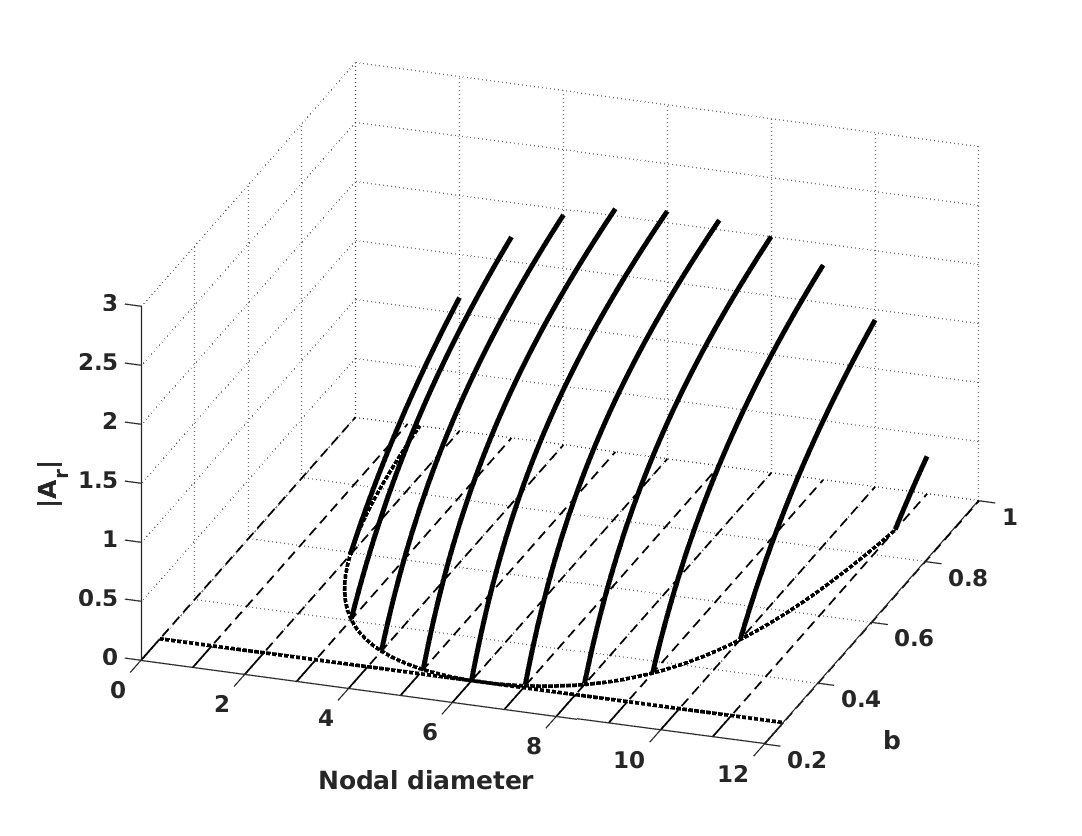
\includegraphics[width = 1\textwidth]{bifurcation_diagram.png}
				\caption{Bifurcation diagram of the periodic solutions for one pure TW (1/2)}
				\label{fig:bifurcation_diagram}
			\end{figure}
		\end{column}
		\begin{column}{0.5\textwidth}
			\begin{figure}[h!]
				\centering
				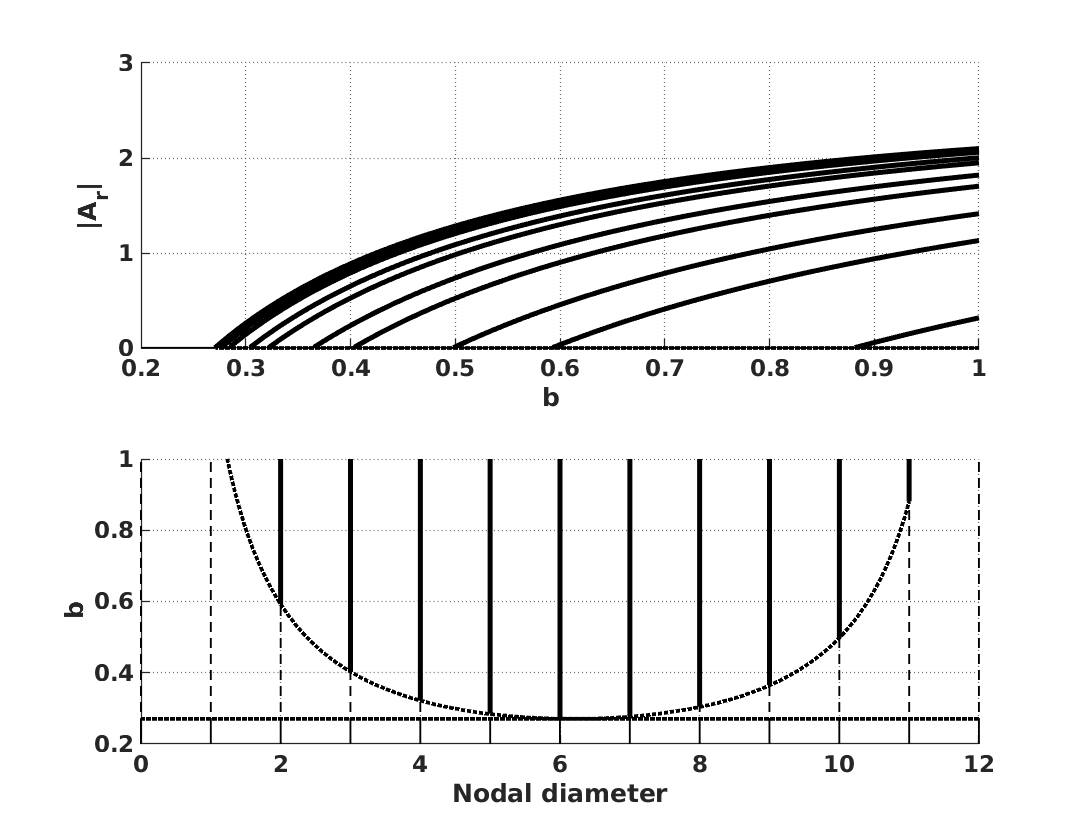
\includegraphics[width = 1\textwidth]{perspective_bif_diag.png}
				\caption{Bifurcation diagram of the periodic solutions for one pure TW (2/2)}
				\label{fig:bifurcation_diagram_details}
			\end{figure}
		\end{column}
	\end{columns}
\end{frame}

\begin{frame}{Stability Analysis}
	\begin{itemize}
		\item Linear stability of a pure TW with wavenumber r: TWr
	\end{itemize}
	\begin{equation}\label{eq:tuned_TW_Basis_linear}
		\begin{split}
			&\frac{\df}{\df \tau}\begin{pmatrix}
				\vdots  \\
				a_{r-1} \\
				a_r     \\
				a_{r+1} \\
				\vdots
			\end{pmatrix}= -\frac{i}{4}Q'(R_r)R_r \left(\begin{pmatrix}
					\vdots  \\
					a_{r-1} \\
					a_r     \\
					a_{r+1} \\
					\vdots
				\end{pmatrix} + \begin{pmatrix}
					\vdots        \\
					\bar{a}_{r+1} \\
					\bar{a}_{r}   \\
					\bar{a}_{r-1} \\
					\vdots
				\end{pmatrix}\right)\\
			&+\begin{bmatrix}
				-\frac{\xi_a^1 - \xi_a^r}{\theta} + i\frac{·\omega_1 - ·\omega_r + \eta_a^1-\eta_a^r}{\theta} &        & \cdots &        & 0                                                                                             \\
				                                                                                              & \ddots &        &        &                                                                                               \\
				\vdots                                                                                        &        & 0      &        & \vdots                                                                                        \\
				                                                                                              &        &        & \ddots &                                                                                               \\
				0                                                                                             &        & \cdots &        & -\frac{\xi_a^N - \xi_a^r}{\theta} + i\frac{·\omega_N - ·\omega_r + \eta_a^N-\eta_a^r}{\theta}
			\end{bmatrix}\begin{pmatrix}
				\vdots  \\
				a_{r-1} \\
				a_r     \\
				a_{r+1} \\
				\vdots
			\end{pmatrix}.
		\end{split}
	\end{equation}
\end{frame}

\begin{frame}{Stability Analysis}
	\begin{columns}
		\begin{column}{0.5\textwidth}
			\begin{itemize}
				\item The damping differences ($\xi_a^j-\xi_a^r $) are small
				\item At the beginning, the growth is given by each $ \xi_a^j + \xi_{mat} $
				\item Decay is much slower because the exponents are one order of magnitude lower
			\end{itemize}
			\begin{figure}[h!]
				\centering
				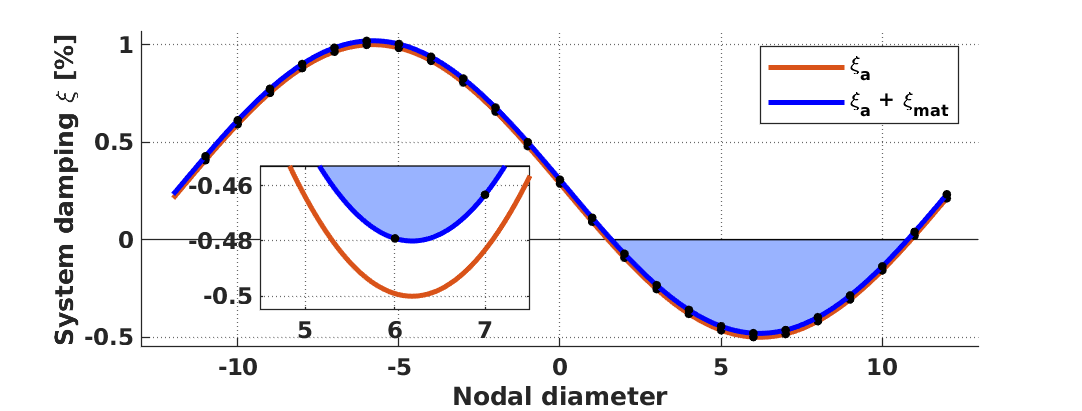
\includegraphics[width = 0.9\textwidth]{aerodynamic_damp_stability.png}
				\label{fig:omega_distributiona22}
				\caption{Aero + structural damping}
			\end{figure}
		\end{column}
		\begin{column}{0.5\textwidth}
			\begin{figure}[h]
				\centering
				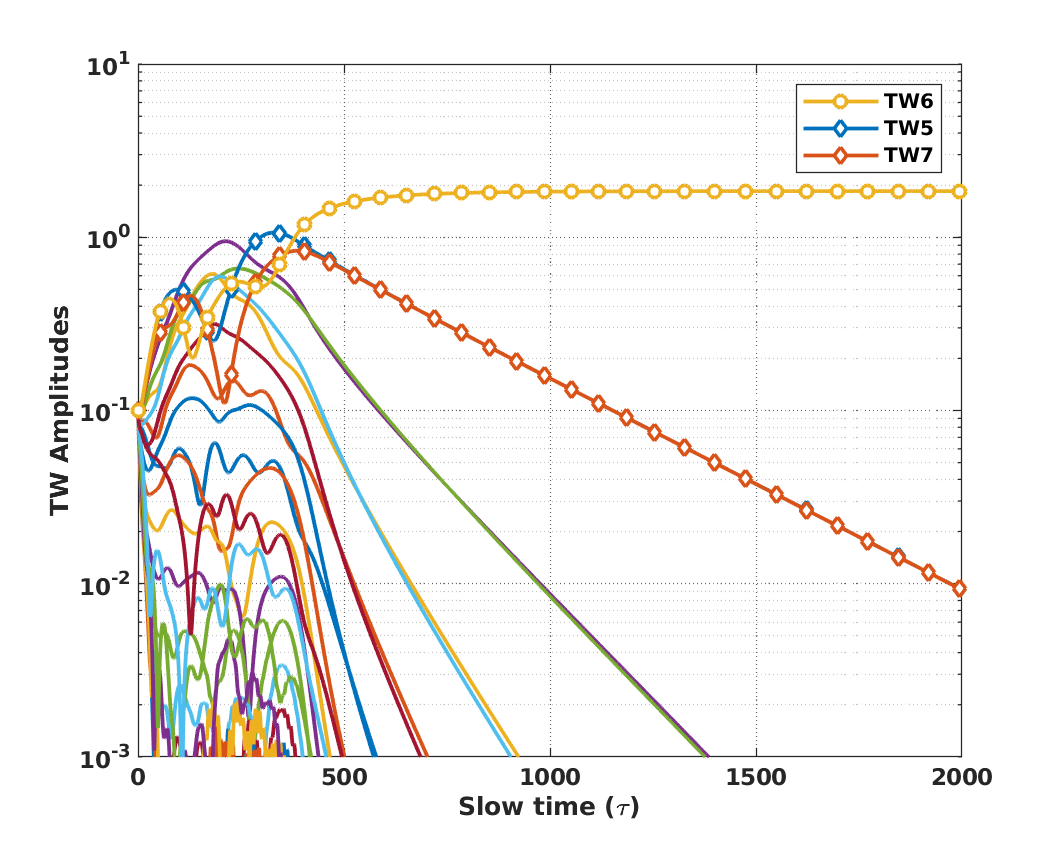
\includegraphics[width = 0.9\textwidth]{log_TW_amplitude.png}
				\caption{TW amplitude evolution (log scale)}
				\label{fig:log_TW_amp_base2}
			\end{figure}
		\end{column}
	\end{columns}
\end{frame}

\begin{frame}{Stability Analysis}
	\begin{columns}
		\begin{column}{0.5\textwidth}
			\begin{itemize}
				\item The periodic solution for the most flutter unstable TW is always stable
				\item Other TWs exhibit an unstable behaviour before becoming stable
				\item New final states could arise from the change in stability of the periodic branches
			\end{itemize}
		\end{column}
		\begin{column}{0.5\textwidth}
			\begin{figure}[h]
				\centering
				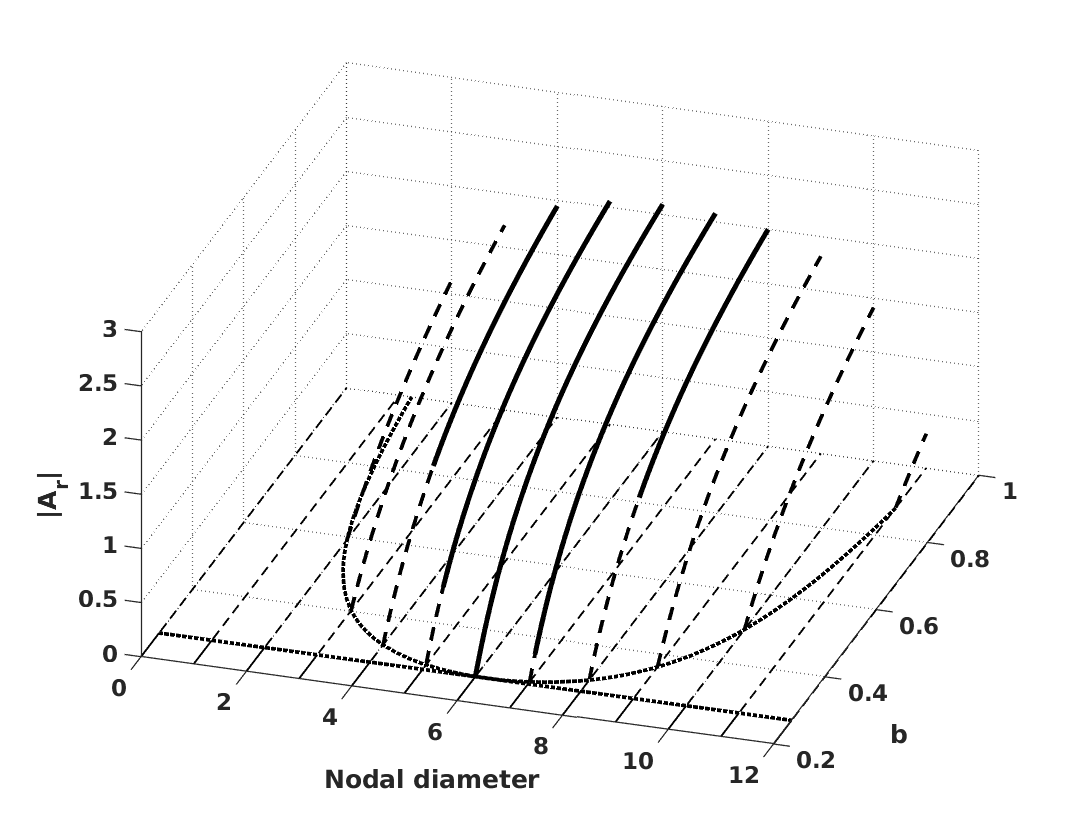
\includegraphics[width = 1\textwidth]{bifurcation_diagram_stable_1.png}
				\caption{Bifurcation diagram with stability (periodic and trivial solutions)}
				\label{fig:log_TW_amp_bas22}
			\end{figure}
		\end{column}
	\end{columns}
\end{frame}
\begin{frame}{Stability Analysis}
	\begin{columns}
		\begin{column}{0.5\textwidth}
			\begin{figure}[h]
				\centering
				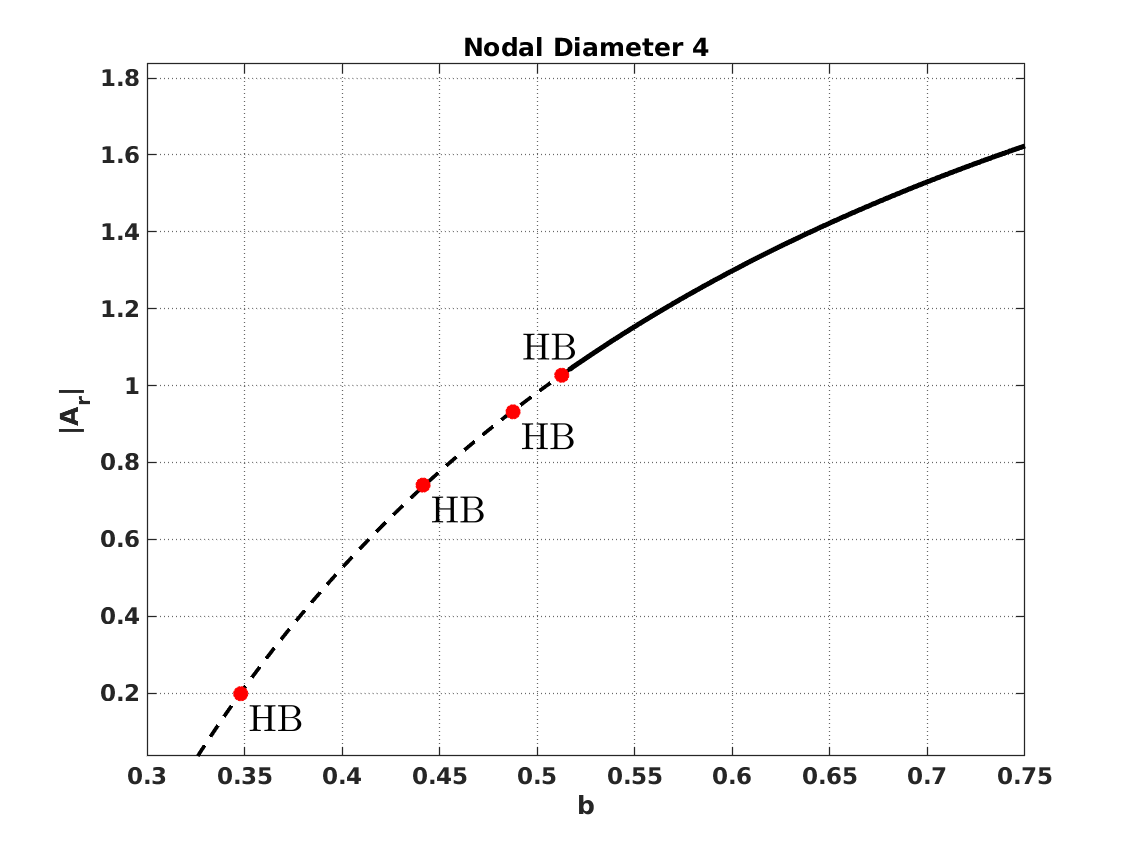
\includegraphics[width = 1\textwidth]{TW4_Bifurcation.png}
				\caption{Bifurcation diagram for TW4}
				\label{fig:log_TW_amp_bas3}
			\end{figure}
		\end{column}
		%			\begin{column}{0.5\textwidth}
		%				\movie[width=6.5cm, height=6.5cm, showcontrols=true]{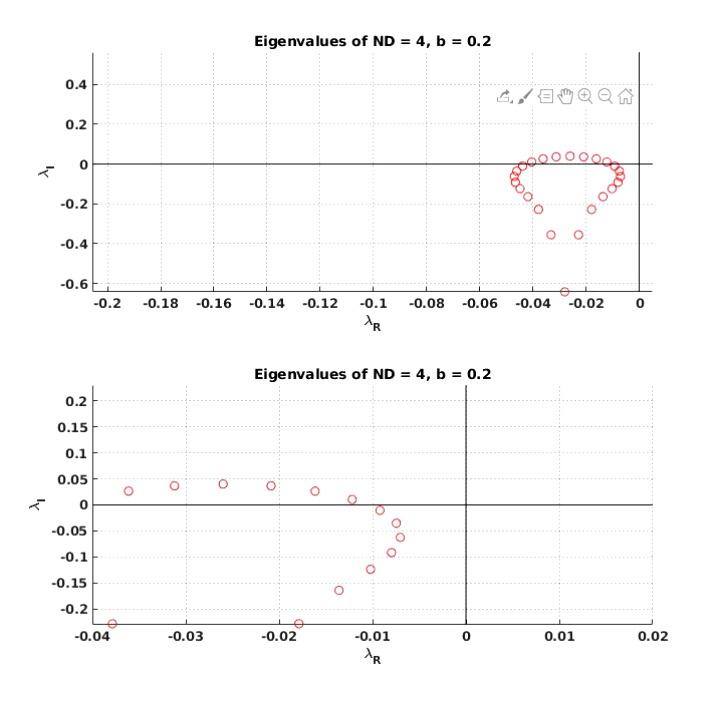
\includegraphics[width=6.5cm, height=6.5cm]{Images/EigenvaluesND4.jpeg}}{Images/EigenvaluesND4.avi}
		%			\end{column}		
	\end{columns}
\end{frame}

\section{Continuation of Quasi-periodic Solutions}

\begin{frame}{Continuation of Quasi-periodic Solutions}
	\begin{columns}
		\begin{column}{0.5\textwidth}
			\begin{itemize}
				\item Numerical continuation is performed to check for new possible final states
				\item The external software AUTO is used
				\item Continuation of the periodic branch with ND = 4 has a new stable quasi-periodic solution
			\end{itemize}
		\end{column}
		\begin{column}{0.5\textwidth}
			\begin{figure}[h!]
				\centering
				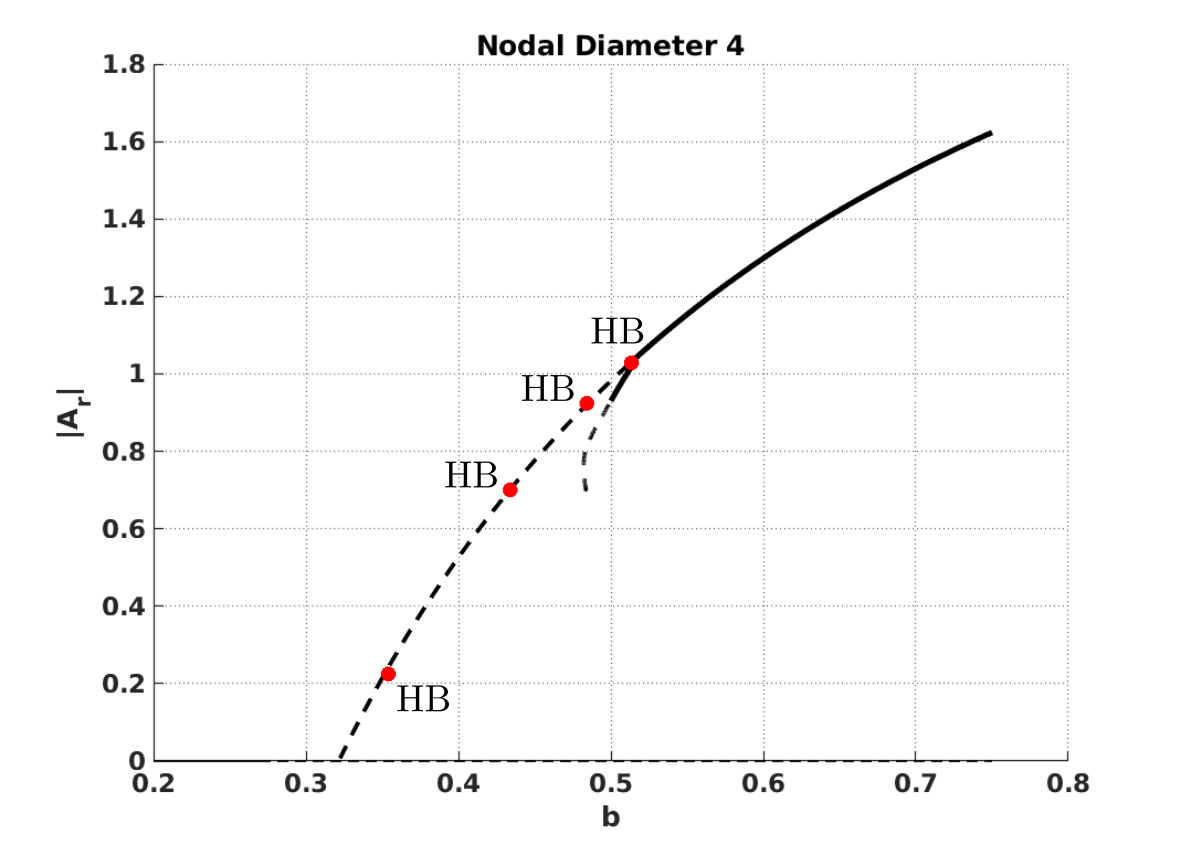
\includegraphics[width = 1\textwidth]{TW4_Bifurcation_newbranch.png}
				\caption{Continuation of the bifurcation diagram for ND = 4 from pure TW4}
				\label{fig:A_4fullbifurcationTW4}
			\end{figure}
		\end{column}
	\end{columns}
\end{frame}


\begin{frame}{Continuation of Quasi-periodic Solutions}
	\begin{columns}
		\begin{column}{0.5\textwidth}
			\begin{figure}[h!]
				\centering
				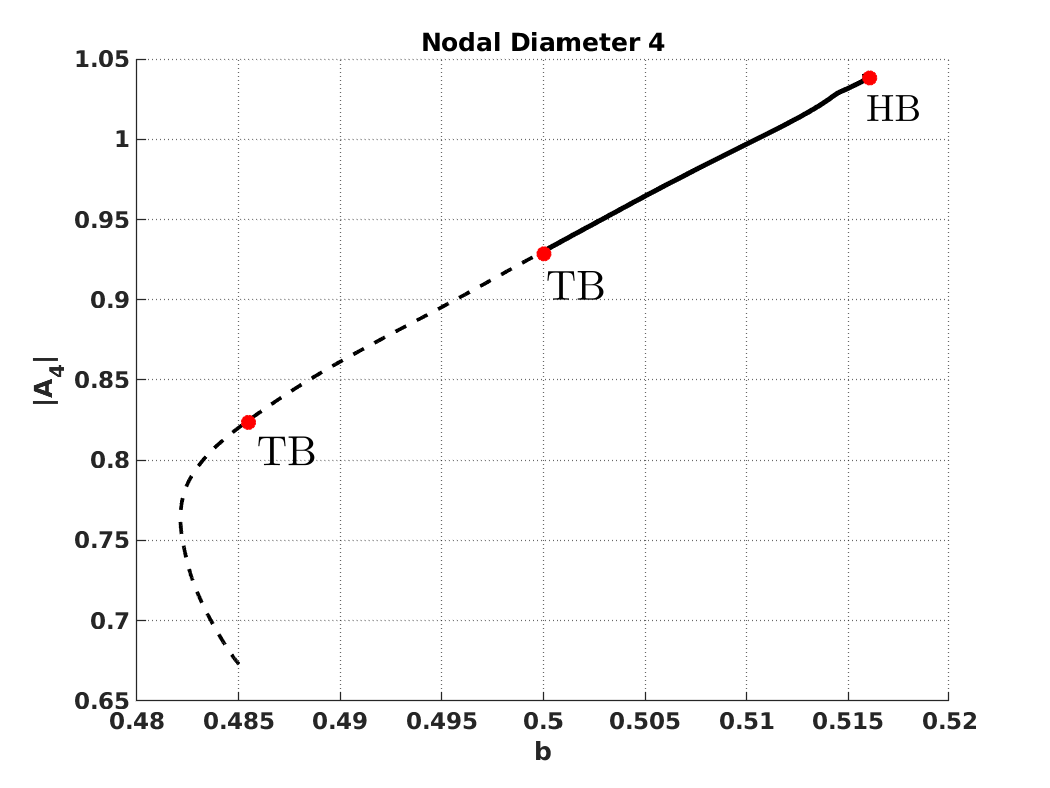
\includegraphics[width = 1\textwidth]{U4TW4.png}
				\caption{Continuation of the bifurcation diagram for ND = 4 from pure TW4}
				\label{fig:A_4newbranchbifurcationTW4}
			\end{figure}
		\end{column}
		\begin{column}{0.5\textwidth}
			\begin{figure}[h!]
				\centering
				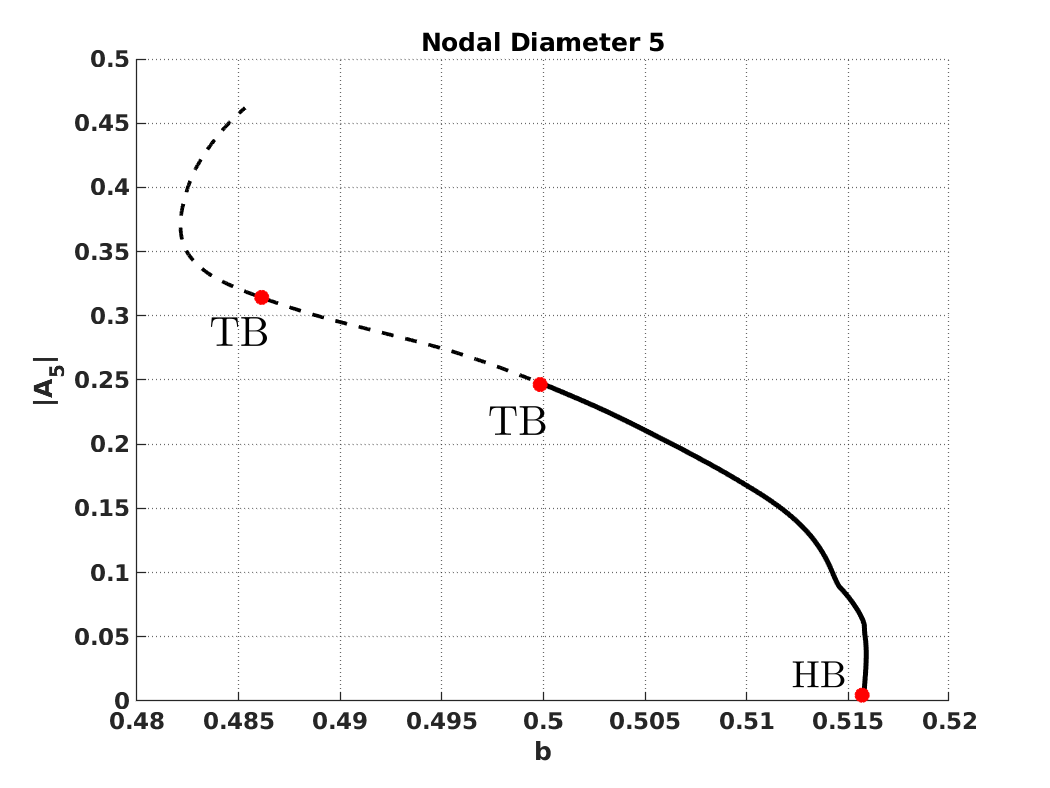
\includegraphics[width = 1\textwidth]{U5TW4.png}
				\caption{Continuation of the bifurcation diagram for ND = 5 from pure TW4}
				\label{fig:A_5newbranchbifurcationTW4}
			\end{figure}
		\end{column}
	\end{columns}
\end{frame}

\begin{frame}{Continuation of Quasi-periodic Solutions}
	\begin{columns}
		\begin{column}{0.5\textwidth}
			\begin{itemize}
				\item This new solution is composed by several TWs
				\item A small variation of the aerodynamic damping greatly increases the amplitude of other TWs (TW5 Amplitude grows to $ \sim 25\% $ of the amplitude of TW4)
				\item New periodic solutions arise from this new branch (Torus Bifurcation)
				\item Continuation from other TWs equilibrium do not present a new stable solution
				\item The quasi-periodic solutions have the effect of a pulse propagating along the bladed-disk
			\end{itemize}
		\end{column}

		\begin{column}{0.45\textwidth}
			\begin{figure}[h!]
				\centering
				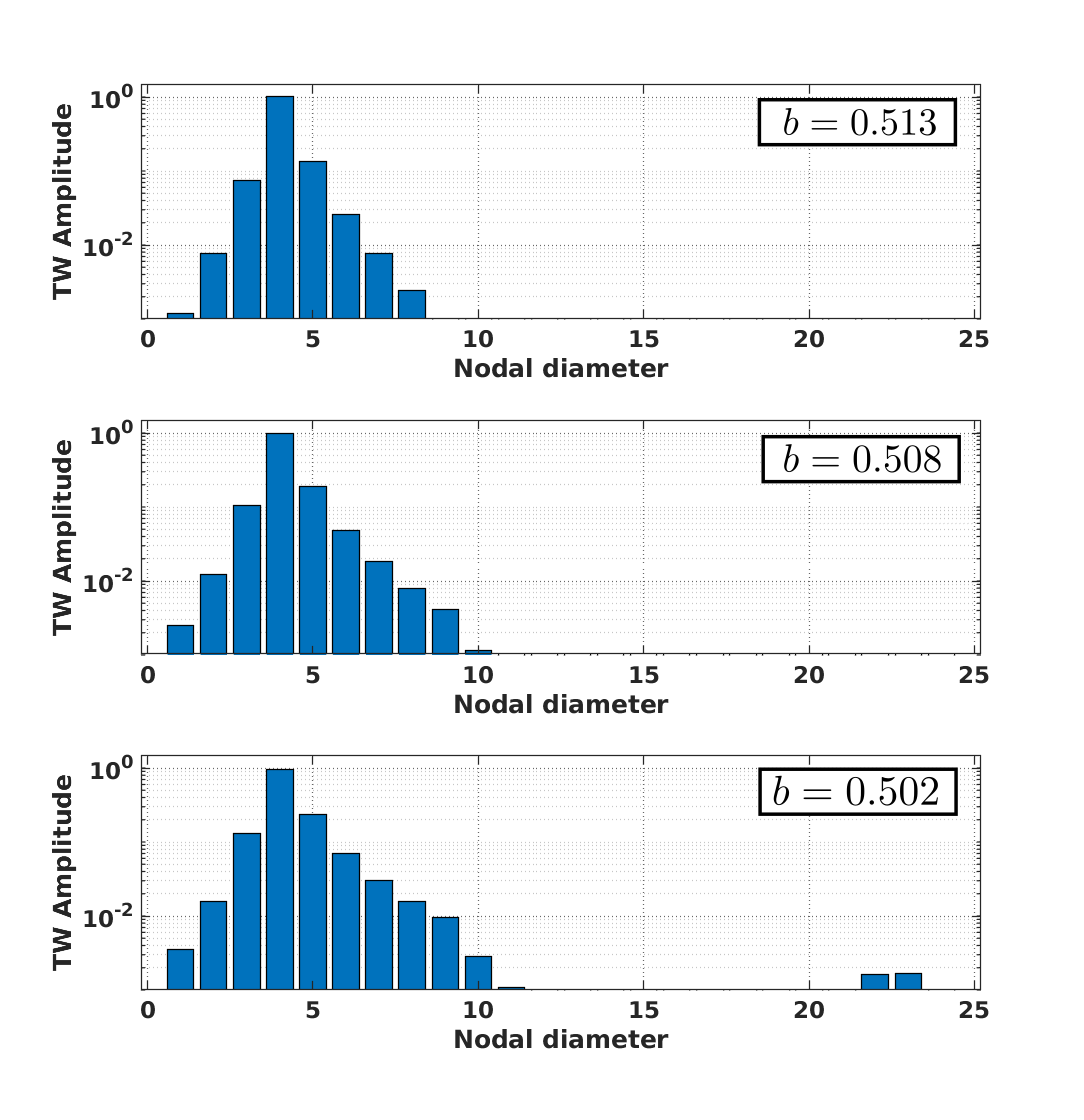
\includegraphics[width = 0.9\textwidth]{TW_amplitudes_multiwave.png}
				\label{fig:Multi-wave_amplitudes}
			\end{figure}
		\end{column}

	\end{columns}
\end{frame}
\begin{frame}{Continuation of Quasi-periodic Solutions}
	\begin{columns}
		\begin{column}{0.5\textwidth}
			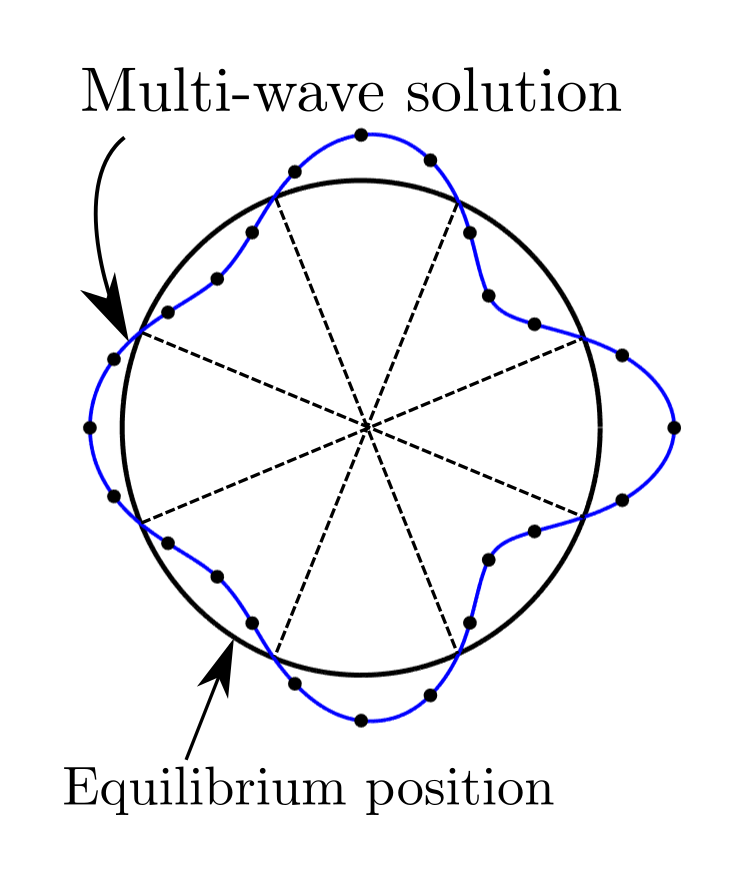
\includegraphics[width=6.2cm,keepaspectratio]{mode_shapesMW.png}
		\end{column}
		%			\begin{column}{0.5\textwidth}
		%				\movie[width=7.3cm, height=4.5cm]{\includegraphics[width=7cm, height=4.7cm]{MultiWave.jpeg}}{Images/MultiWave.avi}
		%			\end{column}		
	\end{columns}
\end{frame}

\section{Conclusions}

\begin{frame}{Conclusions}
	\begin{itemize}
		\item The stability from the trivial solution was determined
		\item Bifurcating from the trivial solution, the periodic solutions for one pure TW were computed and their stability was obtained
		\item Using numerical continuation, a new stable solution were found from the previous pure TW branches. This solution is more complex because is composed by several TW
		\item Previous works showed the final states to be one pure TW (Martel, Corral, Rahul (2015)) or a multi-wave solution (Gross, Krack (2020)). However, they only relied on numerical integration. Generating the bifurcation diagram of the system exploring for stable solutions removes the uncertainty associated with numerical integration.
		\item The multi-wave solution has less maximum displacements amplitude than the pure TW solution.
	\end{itemize}
\end{frame}

\section{References}

\begin{frame}{References}
	\nocite{*}
	\bibliography{biblio}
\end{frame}

\begin{frame}
	\begin{center}
		\LARGE \textbf{Thank you for your attention}
	\end{center}
	\begin{center}
		\vskip 20pt
		\LARGE \textbf{¿Any questions?}
	\end{center}
\end{frame}

\end{document}